% Preamble:
% \usepackage{tikz}

\begin{figure}[ht]
\centering
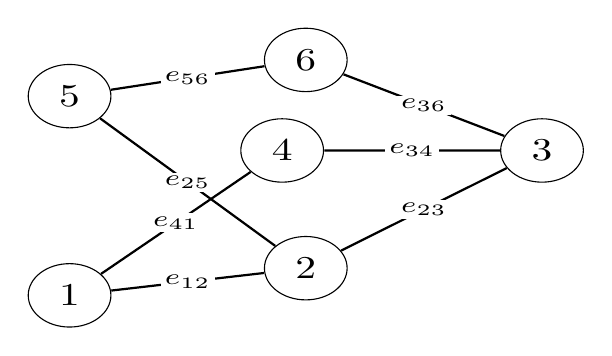
\begin{tikzpicture}[
    xscale=1.5, yscale=1.15, transform shape,
  v/.style={circle, draw, minimum size=7mm},
  e/.style={thick},
  elab/.style={midway, fill=white, inner sep=1pt, font=\scriptsize}
]
% --- 6 vertices (placed "randomly") ---
\node[v] (1) at (0,0)   {$1$};
\node[v] (2) at (2,0.3) {$2$};
\node[v] (3) at (4,1.6) {$3$};
\node[v] (4) at (1.8,1.6) {$4$};
\node[v] (5) at (0,2.2) {$5$};
\node[v] (6) at (2.0,2.6) {$6$};

% --- edges with labels e_{ij} ---
\draw[e] (1)-- node[elab] {$e_{12}$} (2);
\draw[e] (2)-- node[elab] {$e_{23}$} (3);
\draw[e] (3)-- node[elab] {$e_{34}$} (4);
\draw[e] (4)-- node[elab] {$e_{41}$} (1);
\draw[e] (2)-- node[elab] {$e_{25}$} (5);
\draw[e] (5)-- node[elab] {$e_{56}$} (6);
\draw[e] (3)-- node[elab] {$e_{36}$} (6);
\end{tikzpicture}

\caption{A simple undirected graph with vertex set $V=\{1,2,3,4,5,6\}$ and edge set
$E=\{e_{12},e_{23},e_{34},e_{41},e_{25},e_{56},e_{36}\}$.
\textbf{Adjacency (vertex--vertex):} vertices $1$ and $2$ are adjacent because $e_{12}$ joins them; vertices $1$ and $3$ are not adjacent because there is no edge between them.
\textbf{Incidence (edge--vertex):} edge $e_{12}$ is incident to vertices $1$ and $2$ (and is not incident to $3$); the edges incident to vertex $2$ are $e_{12}$, $e_{23}$, and $e_{25}$.}
\label{fig:adjacency-incidence}
\end{figure}
